\section{Anexo}
\label{sec:anexo}
% Opcional, máximo 4 páginas. Figuras o tablas complementarias que no entran en las 8 páginas.

\begin{figure}[!htb]
  \centering
  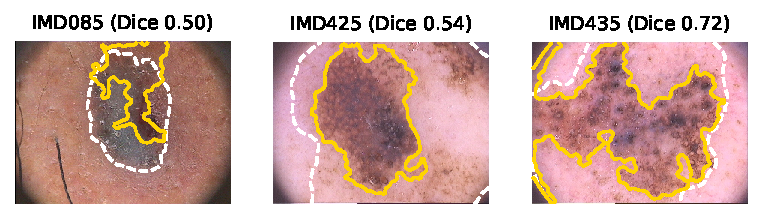
\includegraphics[width=\textwidth]{m3_casos_dificiles}
  \caption{Las imágenes de entrenamiento con peor Dice del método elegido. En blanco punteado, la máscara de PH2; en amarillo, la automática.}
  \label{fig:casos}
\end{figure}

\begin{figure}[!htb]
  \centering
  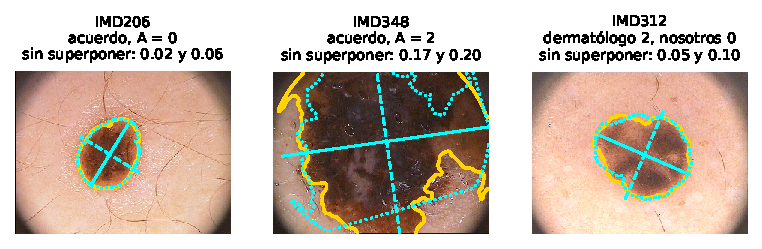
\includegraphics[width=0.85\textwidth]{m4_asimetria_ejemplos}
  \caption{Ejes de simetría y reflejo de la máscara sobre el eje mayor en tres lesiones de entrenamiento. En IMD312 la forma es casi simétrica, pero el pigmento se concentra de un lado, y por eso el dermatólogo puso $A=2$.}
  \label{fig:asimetria}
\end{figure}

\begin{figure}[!htb]
  \centering
  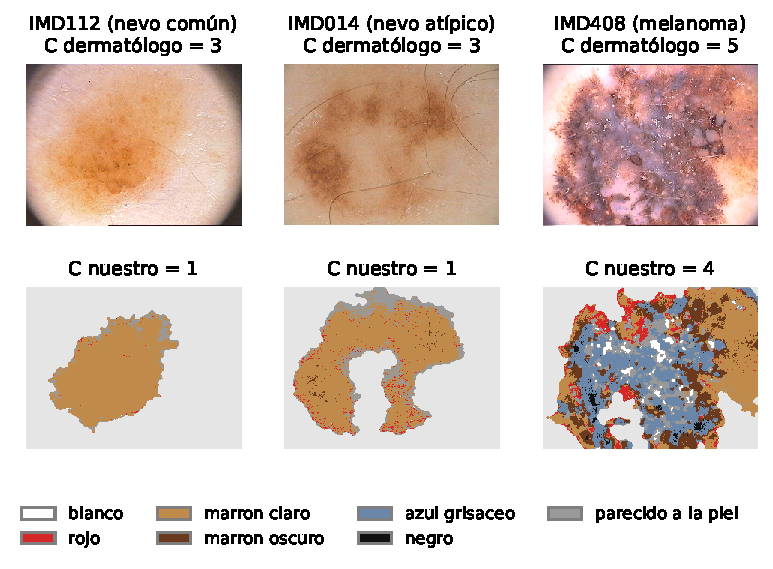
\includegraphics[width=0.7\textwidth]{m4_mapa_colores}
  \caption{Mapa de colores de la lesión con más colores anotados de cada diagnóstico. En los dos nevos casi todo queda como marrón claro, y en el melanoma el blanco y el negro no llegan al 5\,\% de la lesión.}
  \label{fig:colores}
\end{figure}

\begin{table}[!htb]
  \centering\small
  \begin{tabular}{@{}lcccc@{}}
    \toprule
    Color & Zonas & $H$ & $S$ & $V$ \\
    \midrule
    Blanco & 2 & 0,630 & 0,152 & 0,541 \\
    Rojo & 1 & 0,976 & 0,212 & 0,492 \\
    Marrón claro & 12 & 0,083 & 0,249 & 0,452 \\
    Marrón oscuro & 13 & 0,060 & 0,242 & 0,300 \\
    Azul grisáceo & 6 & 0,965 & 0,069 & 0,285 \\
    Negro & 3 & 0,038 & 0,065 & 0,254 \\
    \bottomrule
  \end{tabular}
  \caption{Referencias de color en HSV, con la imagen dividida por el color de la piel, que queda en gris medio ($V=0{,}5$). Cada una es la mediana de las zonas de entrenamiento de ese color.}
  \label{tab:referencias}
\end{table}

\begin{figure}[!htb]
  \centering
  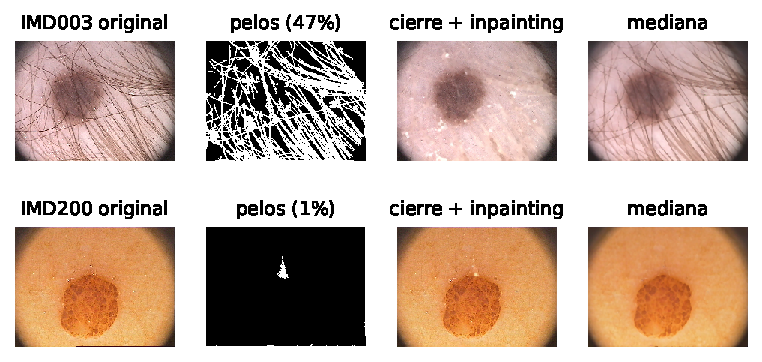
\includegraphics[width=0.85\textwidth]{m1_pelos}
  \caption{Remoción de pelos en una imagen con muchos pelos (IMD003) y en una sin pelos con red de pigmento (IMD200). Se muestran la original, los pelos detectados, el cierre con \emph{inpainting} y el filtro de mediana.}
  \label{fig:pelos}
\end{figure}

\begin{figure}[!htb]
  \centering
  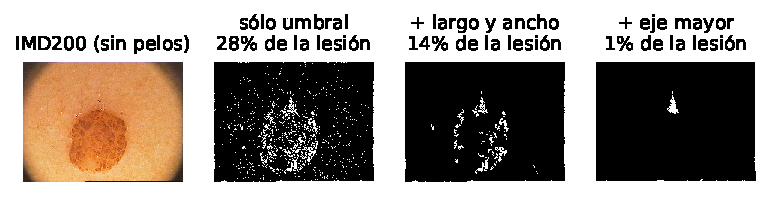
\includegraphics[width=\textwidth]{m1_filtro_forma}
  \caption{Efecto del filtro de forma en la detección de pelos sobre IMD200, que no tiene pelos. Se comparan los candidatos del \emph{black-hat} (sólo umbral), el filtro por largo y ancho y el filtro completo con eje mayor. Se indica la fracción de la lesión marcada como pelo.}
  \label{fig:filtro-forma}
\end{figure}

\begin{figure}[!htb]
  \centering
  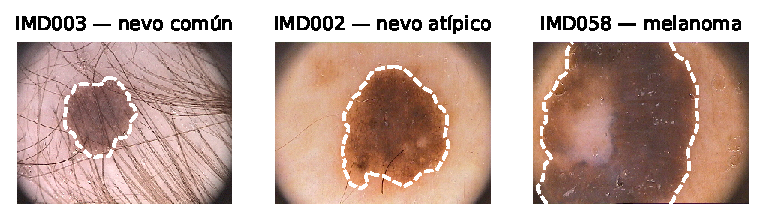
\includegraphics[width=0.75\textwidth]{m0_ejemplos}
  \caption{Un ejemplo de cada diagnóstico de PH2 con el contorno de su máscara manual.}
  \label{fig:ejemplos}
\end{figure}

\begin{figure}[!htb]
  \centering
  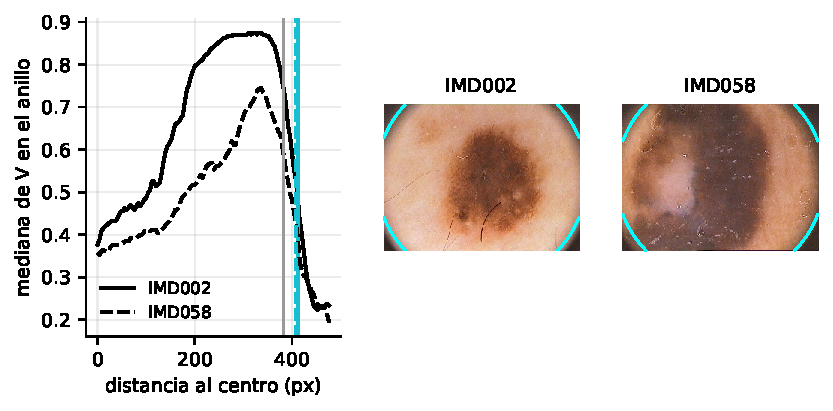
\includegraphics[width=0.75\textwidth]{m1_vineta}
  \caption{Detección del viñeteo. A la izquierda, la mediana del brillo $V$ en anillos concéntricos para una imagen típica (IMD002) y una con la lesión tocando el borde (IMD058), con el radio detectado en líneas verticales. A la derecha, el límite de la zona válida sobre ambas imágenes.}
  \label{fig:vineta}
\end{figure}

\begin{table}[!htb]
  \centering\small
  \begin{tabular}{@{}lll@{}}
    \toprule
    Etapa & Parámetro & Valor \\
    \midrule
    Viñeta & Anillo / umbral / radio mínimo & 4 px / 0,6 del máximo / 0,8 semidiagonal \\
    Pelos  & Elemento estructurante & segmento de 21 px, 12 orientaciones \\
           & Umbral del \emph{black-hat} & 0,10 \\
           & Forma (largo / ancho / eje mayor) & $\ge 60$ px / $\le 8$ px / $\ge 80$ px \\
           & Reconstrucción & \emph{inpainting} de Telea, radio 5 px \\
    Comparación & Filtro de mediana & $9\times9$ por canal \\
    \bottomrule
  \end{tabular}
  \caption{Parámetros del mejoramiento (módulo M1), elegidos con el conjunto de entrenamiento.}
  \label{tab:param-m1}
\end{table}

\begin{table}[!htb]
  \centering\small
  \begin{tabular}{@{}cccccc@{}}
    \toprule
    Calidad & Tasa & PSNR (dB) & PSNR lesión (dB) & SSIM & $\Delta E$ lesión \\
    \midrule
    95 & 8,2   & 41,1 & 40,7 & 0,97 & 1,9 \\
    75 & 23,7  & 35,9 & 34,9 & 0,89 & 2,7 \\
    50 & 39,7  & 34,5 & 33,4 & 0,85 & 3,2 \\
    25 & 67,7  & 32,8 & 31,7 & 0,80 & 3,9 \\
    10 & 121,8 & 29,6 & 28,7 & 0,70 & 5,8 \\
    \bottomrule
  \end{tabular}
  \caption{Compresión JPEG, con la mediana de cada métrica sobre las 140 imágenes de entrenamiento.}
  \label{tab:compresion}
\end{table}

\begin{figure}[!htb]
  \centering
  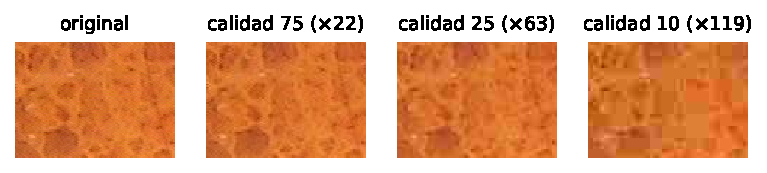
\includegraphics[width=0.85\textwidth]{m2_detalle}
  \caption{Detalle de la red de pigmento de IMD200 en la imagen original y comprimida a calidades 75, 25 y 10 (entre paréntesis, la tasa de compresión).}
  \label{fig:compresion}
\end{figure}

\begin{figure}[!htb]
  \centering
  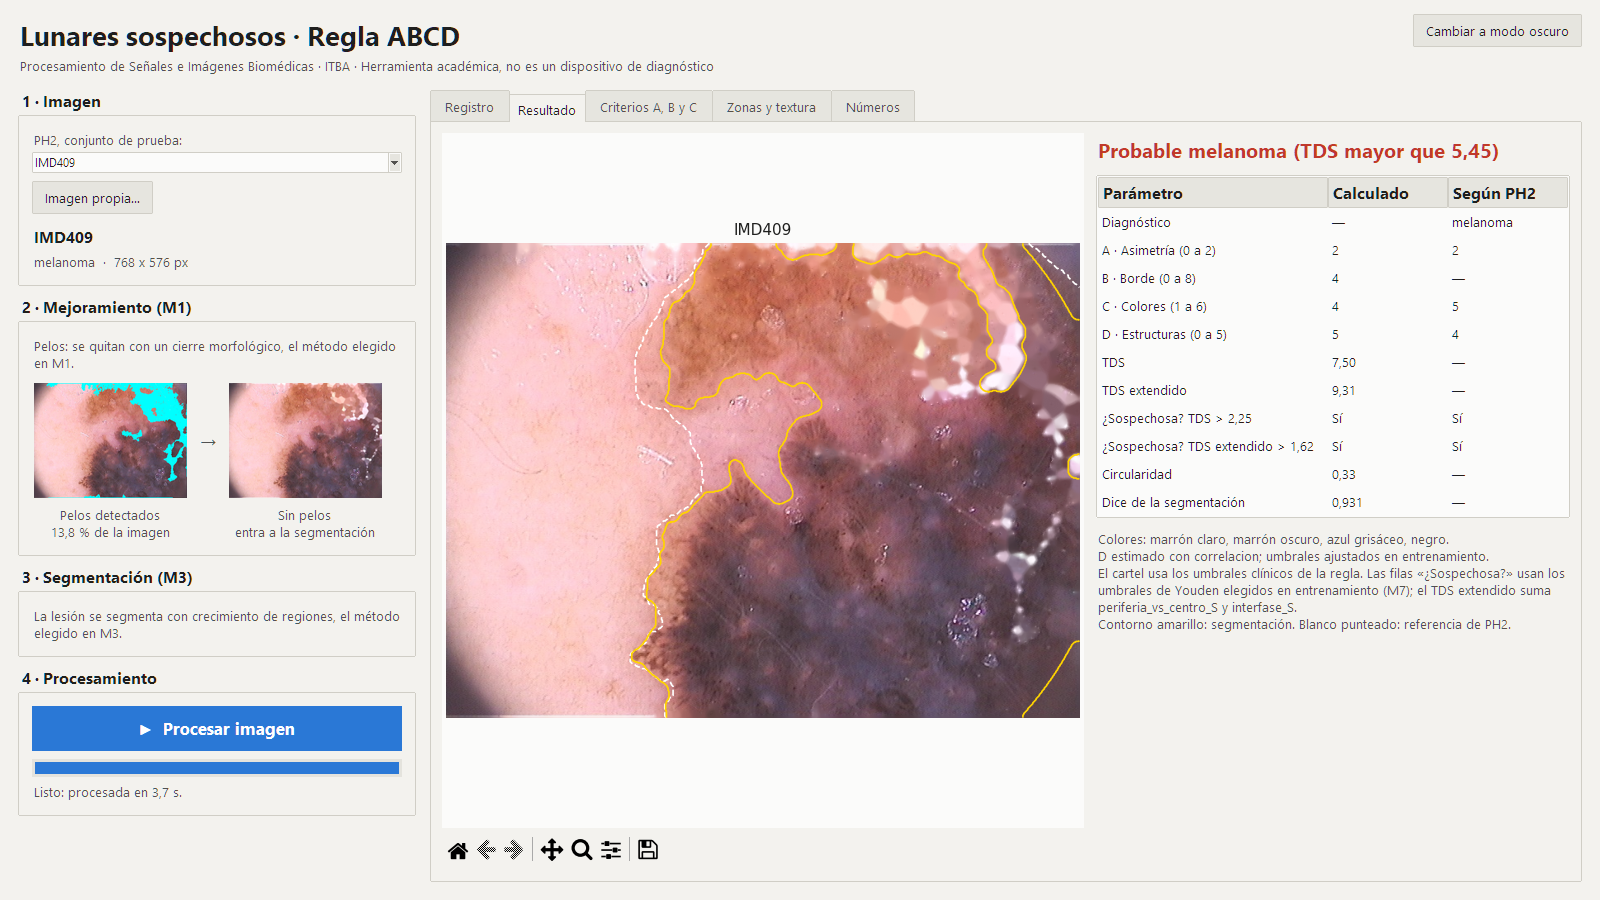
\includegraphics[width=\textwidth]{interfaz}
  \caption{Interfaz gráfica con un melanoma de prueba (IMD409). A la izquierda, los pasos del algoritmo, y a la derecha, la segmentación y la tabla con los criterios calculados junto a los del dermatólogo.}
  \label{fig:interfaz}
\end{figure}

\begin{table}[!htb]
  \centering\footnotesize
  \begin{tabular}{@{}lll@{}}
    \toprule
    Carpeta & Archivo & Contenido \\
    \midrule
    raíz & \texttt{main.py} & Verifica módulos, procesa imágenes y genera resultados \\
    M0 & \texttt{carga\_de\_datos.py} & Lectura de PH2, alcance y partición \\
    M1 & \texttt{mejoramiento.py} & Viñeta y remoción de pelos \\
    M2 & \texttt{compresion.py} & JPEG, tasa de compresión, PSNR y SSIM \\
    M3 & \texttt{segmentacion.py} & Métodos de segmentación, posprocesamiento y Dice \\
    M4 & \texttt{criterios\_abc.py} & Asimetría, borde, colores y circularidad \\
    M5 & \texttt{textura\_criterio\_d.py} & GLCM y criterio D adaptado \\
    M6 & \texttt{zonas\_y\_mapas.py} & Zonas de la lesión y mapas de características \\
    M7 & \texttt{clasificacion\_resultados.py} & TDS, umbrales, métricas y figuras finales \\
    herramientas & \texttt{*.py} & Recorrido completo, verificación y gráficos \\
    interfaz & \texttt{app.py} & Interfaz gráfica \\
    \bottomrule
  \end{tabular}
  \caption{Archivos de Python del repositorio. Cada módulo M$n$ está en \texttt{modulos/m$n$\_\ldots/}.}
  \label{tab:archivos}
\end{table}

\begin{figure}[!htb]
  \centering
  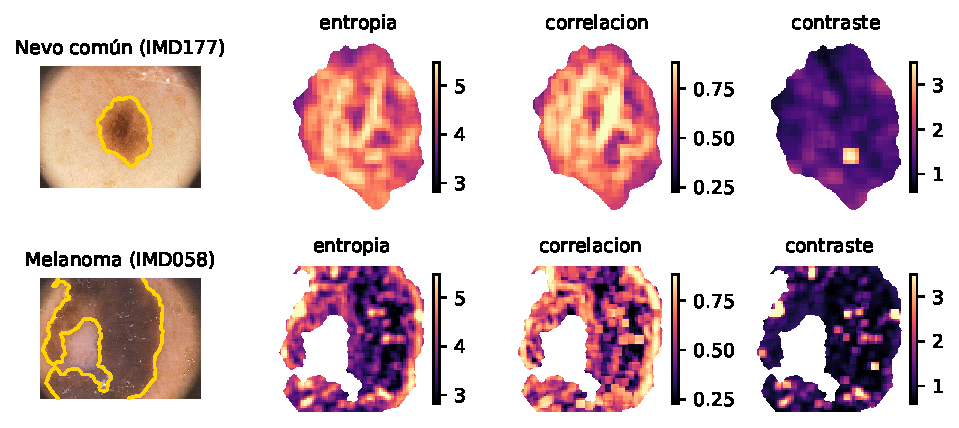
\includegraphics[width=0.78\textwidth]{m6_mapas}
  \caption{Mapas de entropía, correlación y contraste en un nevo común y un melanoma de entrenamiento. El hueco del mapa del melanoma es una zona central clara que la máscara automática dejó afuera.}
  \label{fig:mapas}
\end{figure}
